\section{Performance Methodology}
\label{sec:analysis}

The goal of this project is an analysis of Cornerstone ~\cite{cornerstone} across varying parameter spaces, how the problem maps onto GPU hardware, in the distributed case the communication bottlenecks imposed by the algorithm, and to take advantage of any optimization opportunities that arise. There may be multiple opportunities for improvement as Cornerstone ~\cite{cornerstone} appears to be mostly optimized for the distributed case. Much of the already existing performance analysis in regards to Cornerstone has been for extremely large particle counts with computation distributed across thousands of GPUs. For smaller application spaces such as real-time rendering or simulations on orders of magnitude around or less than $10^8$, a single GPU or a few is likely more optimal due to the constraints imposed by communication costs, against the processing power of the a single GPU, as well as the significant reduction in work that the local case allows. A modern flagship GPU often has at least $40GB$ of DRAM, assuming a particle needs 32 bytes of storage we can fit on the order of 1 billion particles into the GPU. As we will see the overhead for distributing work is not trivial. Due to technical constraints, our preliminary results and analysis operate using only a single node with with 1 or 2 peer ranks each with their own GPU. However these type of workloads involving only modest numbers of GPUs are not uncommon especially in applications like computer aided engineering, and analysis on these workloads may yield useful conclusions for a number of use cases.

\subsection{Code}
To evaluate the Cornerstone octree construction method under realistic conditions, we developed a configurable batch generation pipeline that sweeps over a matrix of particle distributions, particle counts, and perturbation magnitudes. This hooks into our testing harness that runs the simulation with the ability to select between using GPUs or CPUs, the local only or distributed MPI case using a global tree and focus tree, and other parameters of interest. This is flexible enough to allow us to generate any metrics of interest in the future and has already allowed us to gather the results discussed in \ref{sec:results}.

We created the necessary Python scripts to generate the initial particle distributions and the perturbed versions of the distribution used throughout this paper. This includes saving those distributions to HDF5 files, which could then be loaded in the C++ parts of the codebase to generate their corresponding octrees whether it be initial construction or a rebalance to an already existing octree. This allowed us to test many different types of distributions and their corresponding perturbation if they had one. Tooling to instrument sections of interest is done using NVIDIA Tooling Extensions (NVTX). We instrumented our code to highlight important metrics at a relatively coarse level so that we could observe the primary steps necessary to building the Octree and focus our attention on bottlenecks. The program "perf" was also used to generate profiles on the CPU, which were also used to identify bottlenecks.

\subsection{Distribution Generators}
All initial particle distributions are confined to the cube domain $[-1,1]^3$, where all distributions are as large as the domain.
Six initial particle distributions are used:

\begin{enumerate}
    \item \textbf{\texttt{uniform\_initial}}: Samples particles uniformly at random from the domain.
    \item \textbf{\texttt{pancake\_initial}}: A cylindrical distribution along the Z-axis where the Z-axis is strongly compressed, as to resemble a disk, frisbee, or (as the name suggests) pancake.
    \item \textbf{\texttt{pancake\_initial\_tilted}}: Same as the pancake but tilted off-axis, so the thin dimension is no longer aligned with a coordinate plane.
    \item \textbf{\texttt{filament\_z\_initial}}: A one-dimensional filament aligned along the $z$-axis, characterized by the parametric equation: (0, 0, t).
    \item \textbf{\texttt{filament\_yz\_initial}}: A filament lying in the $yz$-plane, anisotropic in two directions, characterized by the parametric equation: (0, t, t).
    \item \textbf{\texttt{filament\_xyz\_initial}}: A filament oriented along the domain diagonal, anisotropic in all three coordinate directions simultaneously, characterized by the parametric equation: (t, t, t).
\end{enumerate}

By analyzing 1D, 2D, and 3D manifolds that are or are not axis-aligned, a wide variety of behavior can be observed after applying perturbations. Because the perturbation distribution is 3-dimensional, the various distributions will have their unique attributes degraded as the perturbation magnitude increases.  

% \begin{figure*}[ht]
%     \centering
%     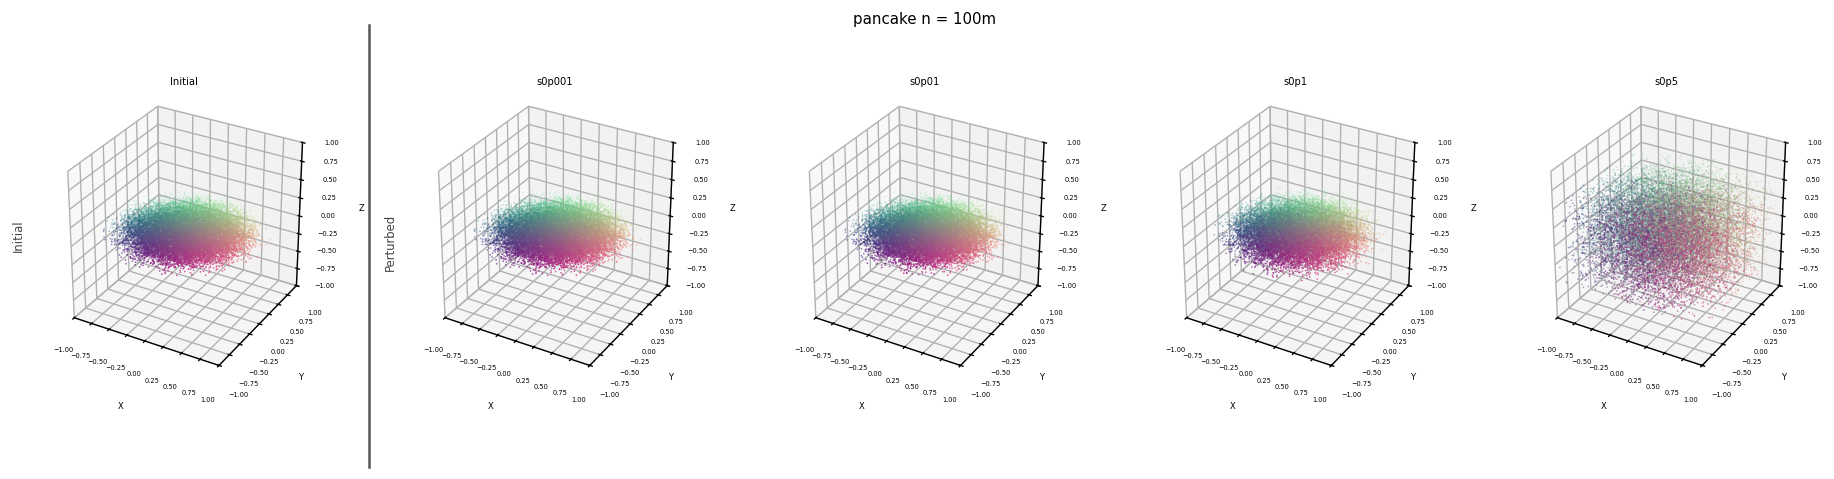
\includegraphics[width=\textwidth]{visualizations/pancake/n100m/pancake_n100m_positions.png}\\[0.5em]
%     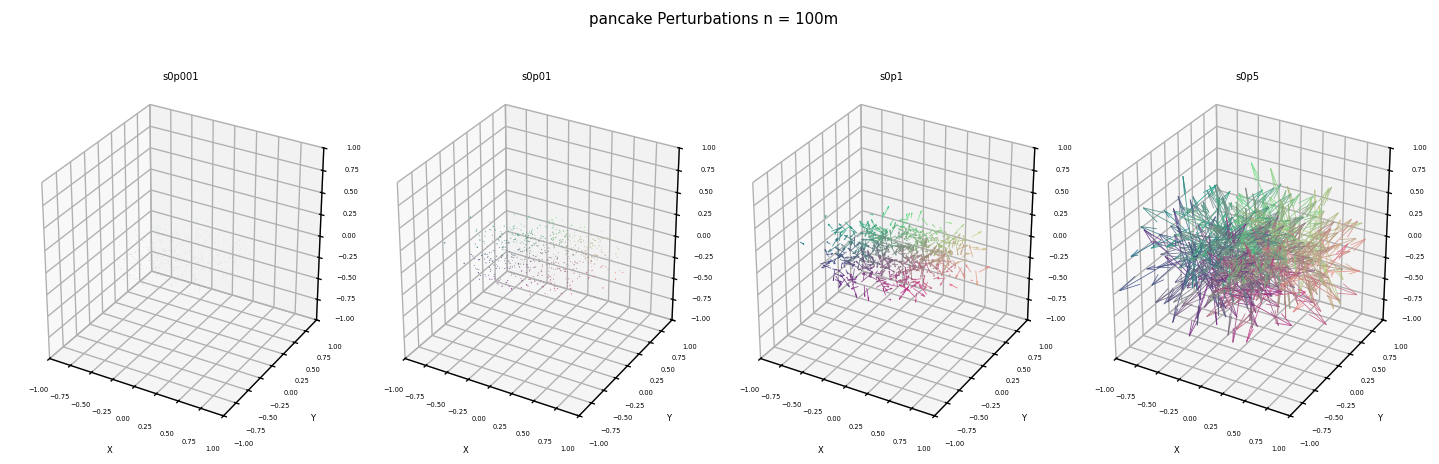
\includegraphics[width=\textwidth]{visualizations/pancake/n100m/pancake_n100m_perturbations.png}
%     \caption{Pancake distribution with $10^8$ particles. Top: initial and final positions. Bottom: perturbation vectors.}
%     \label{fig:pancake_vis}
% \end{figure*}

% \begin{figure*}[ht]
%     \centering
%     
\includegraphics[width=\textwidth]{visualizations/pancake_initial_tilted/n100m/pancake_initial_tilted_n100m_positions.png}\\[0.5em]
%     
\includegraphics[width=\textwidth]{visualizations/pancake_initial_tilted/n100m/pancake_initial_tilted_n100m_perturbations.png}
%     \caption{Tilted pancake distribution with $10^8$ particles. Top: initial and final positions. Bottom: perturbation vectors.}
%     \label{fig:pancake_tilted_vis}
% \end{figure*}

% \begin{figure*}[ht]
%     \centering
%     
\includegraphics[width=\textwidth]{visualizations/filament_xyz/n100m/filament_xyz_n100m_positions.png}\\[0.5em]
%     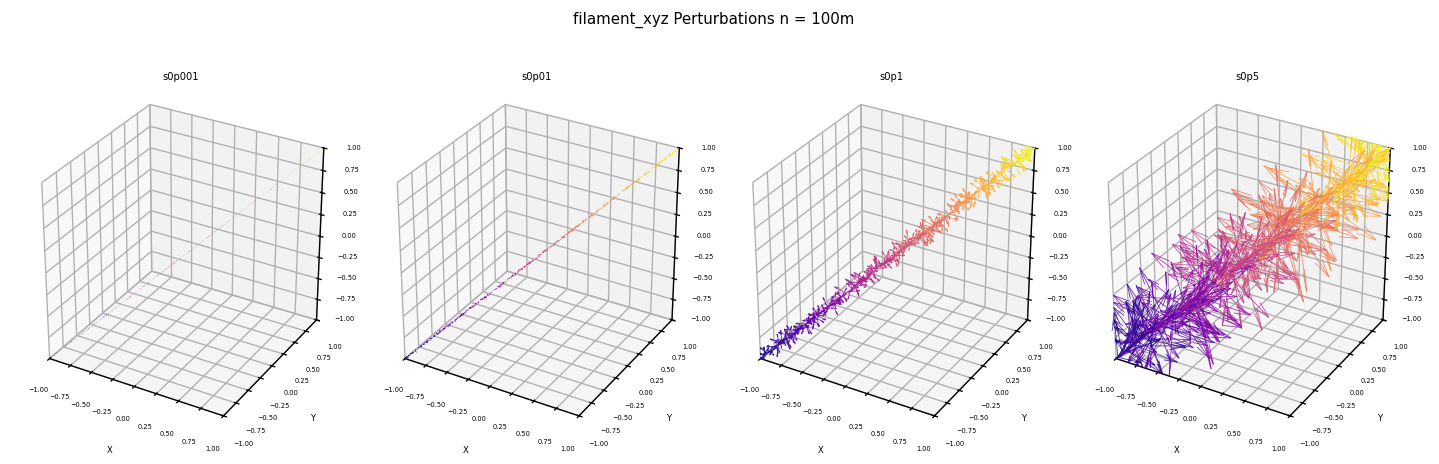
\includegraphics[width=\textwidth]{visualizations/filament_xyz/n100m/filament_xyz_n100m_perturbations.png}
%     \caption{Filament XYZ distribution with $10^8$ particles. Top: initial and final positions. Bottom: perturbation vectors.}
%     \label{fig:filament_xyz_vis}
% \end{figure*}

\begin{figure*}[ht]
    \centering
    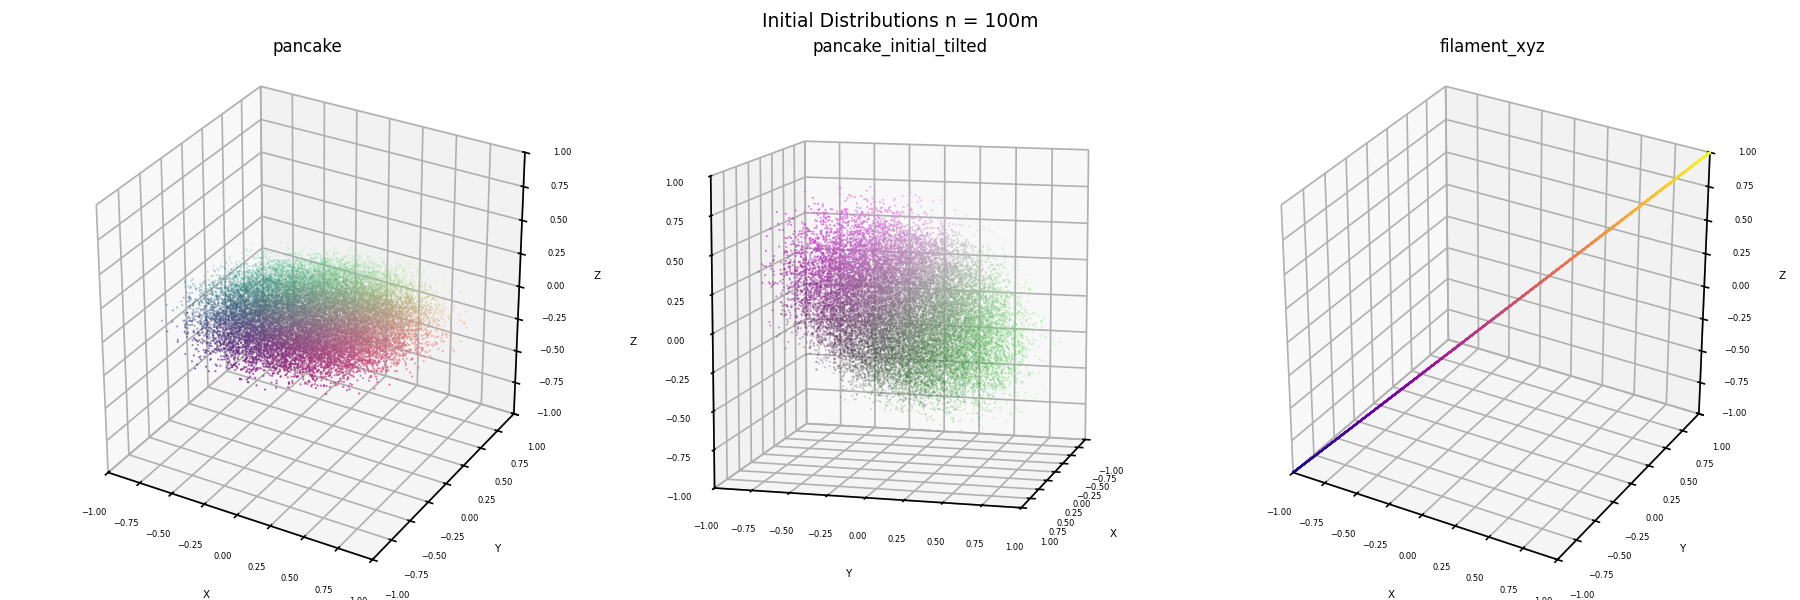
\includegraphics[width=\textwidth]{initial_dist/initial_distributions_n100m.png}
    \caption{Initial particle distributions with $10^8$ particles.}
    \label{fig:initial_distributions}
\end{figure*}

\subsection{Perturbation Model}

After the initial distribution is generated, a perturbation vector is applied to simulate particle motion between timesteps. The perturbation function draws each displacement component independently from $\mathcal{U}(-s, +s)$ where $s$ is the scale factor. Particles that move outside the domain after perturbation are truncated to the boundary (\texttt{out\_of\_bounds = `truncate'}). Four perturbation scales are used:

\begin{itemize}
    \item $s = 0.001$: Very small perturbation; particles barely move relative to the domain.
    \item $s = 0.01$\phantom{0}: Moderate perturbation; noticeable displacement but locally coherent.
    \item $s = 0.1$\phantom{00}: Large perturbation; significant displacement triggering substantial tree restructuring.
    \item $s = 0.5$\phantom{00}: Very large perturbation; particles may traverse a large fraction of the domain.
\end{itemize}

\subsection{Runtime Configuration}

The Cornerstone framework accepts several runtime parameters via the command line:

\begin{itemize}
    \item \texttt{--bucket-size-global}: Maximum number of particles per leaf node in the global octree (default: 1024).
    \item \texttt{--bucket-size-focus}: Maximum number of particles per leaf node in the focused octree (default: 64).
    \item \texttt{--theta}: The multipole acceptance criterion (MAC) parameter controlling the accuracy/performance tradeoff (default: 0.6).
    \item \texttt{--gpu}: Flag to enable GPU-accelerated octree construction.
    \item \texttt{--lets}: Flag to enable Cornerstone ~\cite{cornerstone} to use Locally Essential Trees and communicate with peer ranks rather than use only local trees.
\end{itemize}

% No rotations were applied (\texttt{rotations = None}).

\subsection{Test Configurations}

The full sweep comprises $6$ distributions $\times$ $5$ particle counts $\times$ $4$ perturbation scales $= 120$ configurations. There were also several tests run independently of this parameter sweep to gather general metrics which used a uniform distribution of particles on the unit cube.

\subsection{Machines}
For initial results on we used \href{https://www.cloudlab.us/}{CloudLab} to gain access to GPUs allowing us to get on a node with 4 V100s; 
For all the results presented in \ref{sec:results} we used a c4130 node on the CloudLab Wisconsin cluster. The node had four NVIDIA Tesla V100 GPUs. Each GPU had 16GB of memory in an SXM2 configuration with 900 GB/sec of peak memory bandwidth. A single V100 has 84 Streaming multiprocessors each with 64 FP32 cores, 64 INT32 cores, and 32 FP64 cores.

% --- Uniform ---
% \begin{table*}[ht]
%     \centering
%     \caption{\texttt{uniform\_initial} results.}
%     \label{tab:uniform_results}
%     \begin{tabular}{|c|c|c|c|c|}
%         \hline
%         \textbf{$N$} & \textbf{Scale} & \textbf{Build (ms)} & \textbf{Rebalance (ms)} & \textbf{Depth} \\
%         \hline
%         $10^4$ & $0.001$ & & & \\
%         $10^4$ & $0.01$  & & & \\
%         $10^4$ & $0.1$   & & & \\
%         $10^4$ & $0.5$   & & & \\
%         \hline
%         $10^5$ & $0.001$ & & & \\
%         $10^5$ & $0.01$  & & & \\
%         $10^5$ & $0.1$   & & & \\
%         $10^5$ & $0.5$   & & & \\
%         \hline
%         $10^6$ & $0.001$ & & & \\
%         $10^6$ & $0.01$  & & & \\
%         $10^6$ & $0.1$   & & & \\
%         $10^6$ & $0.5$   & & & \\
%         \hline
%         $10^7$ & $0.001$ & & & \\
%         $10^7$ & $0.01$  & & & \\
%         $10^7$ & $0.1$   & & & \\
%         $10^7$ & $0.5$   & & & \\
%         \hline
%         $10^8$ & $0.001$ & & & \\
%         $10^8$ & $0.01$  & & & \\
%         $10^8$ & $0.1$   & & & \\
%         $10^8$ & $0.5$   & & & \\
%         \hline
%     \end{tabular}
% \end{table*}

% % --- Pancake ---
% \begin{table*}[ht]
%     \centering
%     \caption{\texttt{pancake\_initial} results.}
%     \label{tab:pancake_results}
%     \begin{tabular}{|c|c|c|c|c|}
%         \hline
%         \textbf{$N$} & \textbf{Scale} & \textbf{Build (ms)} & \textbf{Rebalance (ms)} & \textbf{Depth} \\
%         \hline
%         $10^4$ & $0.001$ & & & \\
%         $10^4$ & $0.01$  & & & \\
%         $10^4$ & $0.1$   & & & \\
%         $10^4$ & $0.5$   & & & \\
%         \hline
%         $10^5$ & $0.001$ & & & \\
%         $10^5$ & $0.01$  & & & \\
%         $10^5$ & $0.1$   & & & \\
%         $10^5$ & $0.5$   & & & \\
%         \hline
%         $10^6$ & $0.001$ & & & \\
%         $10^6$ & $0.01$  & & & \\
%         $10^6$ & $0.1$   & & & \\
%         $10^6$ & $0.5$   & & & \\
%         \hline
%         $10^7$ & $0.001$ & & & \\
%         $10^7$ & $0.01$  & & & \\
%         $10^7$ & $0.1$   & & & \\
%         $10^7$ & $0.5$   & & & \\
%         \hline
%         $10^8$ & $0.001$ & & & \\
%         $10^8$ & $0.01$  & & & \\
%         $10^8$ & $0.1$   & & & \\
%         $10^8$ & $0.5$   & & & \\
%         \hline
%     \end{tabular}
% \end{table*}

% % --- Pancake Tilted ---
% \begin{table*}[ht]
%     \centering
%     \caption{\texttt{pancake\_initial\_tilted} results.}
%     \label{tab:pancake_tilted_results}
%     \begin{tabular}{|c|c|c|c|c|}
%         \hline
%         \textbf{$N$} & \textbf{Scale} & \textbf{Build (ms)} & \textbf{Rebalance (ms)} & \textbf{Depth} \\
%         \hline
%         $10^4$ & $0.001$ & & & \\
%         $10^4$ & $0.01$  & & & \\
%         $10^4$ & $0.1$   & & & \\
%         $10^4$ & $0.5$   & & & \\
%         \hline
%         $10^5$ & $0.001$ & & & \\
%         $10^5$ & $0.01$  & & & \\
%         $10^5$ & $0.1$   & & & \\
%         $10^5$ & $0.5$   & & & \\
%         \hline
%         $10^6$ & $0.001$ & & & \\
%         $10^6$ & $0.01$  & & & \\
%         $10^6$ & $0.1$   & & & \\
%         $10^6$ & $0.5$   & & & \\
%         \hline
%         $10^7$ & $0.001$ & & & \\
%         $10^7$ & $0.01$  & & & \\
%         $10^7$ & $0.1$   & & & \\
%         $10^7$ & $0.5$   & & & \\
%         \hline
%         $10^8$ & $0.001$ & & & \\
%         $10^8$ & $0.01$  & & & \\
%         $10^8$ & $0.1$   & & & \\
%         $10^8$ & $0.5$   & & & \\
%         \hline
%     \end{tabular}
% \end{table*}

% % --- Filament Z ---
% \begin{table*}[ht]
%     \centering
%     \caption{\texttt{filament\_z\_initial} results.}
%     \label{tab:filament_z_results}
%     \begin{tabular}{|c|c|c|c|c|}
%         \hline
%         \textbf{$N$} & \textbf{Scale} & \textbf{Build (ms)} & \textbf{Rebalance (ms)} & \textbf{Depth} \\
%         \hline
%         $10^4$ & $0.001$ & & & \\
%         $10^4$ & $0.01$  & & & \\
%         $10^4$ & $0.1$   & & & \\
%         $10^4$ & $0.5$   & & & \\
%         \hline
%         $10^5$ & $0.001$ & & & \\
%         $10^5$ & $0.01$  & & & \\
%         $10^5$ & $0.1$   & & & \\
%         $10^5$ & $0.5$   & & & \\
%         \hline
%         $10^6$ & $0.001$ & & & \\
%         $10^6$ & $0.01$  & & & \\
%         $10^6$ & $0.1$   & & & \\
%         $10^6$ & $0.5$   & & & \\
%         \hline
%         $10^7$ & $0.001$ & & & \\
%         $10^7$ & $0.01$  & & & \\
%         $10^7$ & $0.1$   & & & \\
%         $10^7$ & $0.5$   & & & \\
%         \hline
%         $10^8$ & $0.001$ & & & \\
%         $10^8$ & $0.01$  & & & \\
%         $10^8$ & $0.1$   & & & \\
%         $10^8$ & $0.5$   & & & \\
%         \hline
%     \end{tabular}
% \end{table*}

% % --- Filament YZ ---
% \begin{table*}[ht]
%     \centering
%     \caption{\texttt{filament\_yz\_initial} results.}
%     \label{tab:filament_yz_results}
%     \begin{tabular}{|c|c|c|c|c|}
%         \hline
%         \textbf{$N$} & \textbf{Scale} & \textbf{Build (ms)} & \textbf{Rebalance (ms)} & \textbf{Depth} \\
%         \hline
%         $10^4$ & $0.001$ & & & \\
%         $10^4$ & $0.01$  & & & \\
%         $10^4$ & $0.1$   & & & \\
%         $10^4$ & $0.5$   & & & \\
%         \hline
%         $10^5$ & $0.001$ & & & \\
%         $10^5$ & $0.01$  & & & \\
%         $10^5$ & $0.1$   & & & \\
%         $10^5$ & $0.5$   & & & \\
%         \hline
%         $10^6$ & $0.001$ & & & \\
%         $10^6$ & $0.01$  & & & \\
%         $10^6$ & $0.1$   & & & \\
%         $10^6$ & $0.5$   & & & \\
%         \hline
%         $10^7$ & $0.001$ & & & \\
%         $10^7$ & $0.01$  & & & \\
%         $10^7$ & $0.1$   & & & \\
%         $10^7$ & $0.5$   & & & \\
%         \hline
%         $10^8$ & $0.001$ & & & \\
%         $10^8$ & $0.01$  & & & \\
%         $10^8$ & $0.1$   & & & \\
%         $10^8$ & $0.5$   & & & \\
%         \hline
%     \end{tabular}
% \end{table*}

% % --- Filament XYZ ---
% \begin{table*}[ht]
%     \centering
%     \caption{\texttt{filament\_xyz\_initial} results.}
%     \label{tab:filament_xyz_results}
%     \begin{tabular}{|c|c|c|c|c|}
%         \hline
%         \textbf{$N$} & \textbf{Scale} & \textbf{Build (ms)} & \textbf{Rebalance (ms)} & \textbf{Depth} \\
%         \hline
%         $10^4$ & $0.001$ & & & \\
%         $10^4$ & $0.01$  & & & \\
%         $10^4$ & $0.1$   & & & \\
%         $10^4$ & $0.5$   & & & \\
%         \hline
%         $10^5$ & $0.001$ & & & \\
%         $10^5$ & $0.01$  & & & \\
%         $10^5$ & $0.1$   & & & \\
%         $10^5$ & $0.5$   & & & \\
%         \hline
%         $10^6$ & $0.001$ & & & \\
%         $10^6$ & $0.01$  & & & \\
%         $10^6$ & $0.1$   & & & \\
%         $10^6$ & $0.5$   & & & \\
%         \hline
%         $10^7$ & $0.001$ & & & \\
%         $10^7$ & $0.01$  & & & \\
%         $10^7$ & $0.1$   & & & \\
%         $10^7$ & $0.5$   & & & \\
%         \hline
%         $10^8$ & $0.001$ & & & \\
%         $10^8$ & $0.01$  & & & \\
%         $10^8$ & $0.1$   & & & \\
%         $10^8$ & $0.5$   & & & \\
%         \hline
%     \end{tabular}
% \end{table*}
